El objetivo de este capítulo es demostrar las partes importantes o de interés de la implementación y como se ha logrado la realización de lo estipulado en capítulos anteriores.

\section{El controlador}
Como se ha comentado en capítulos anteriores, la mayoría de comandos se aprovecha de los comandos ya proporcionados por \verb|gh|. Como es el caso de \verb|gh edu install|. Después de determinar si la extensión es \emph{first-party} o \emph{third-party} (extensión independiente de la organización \verb|gh-cli-for-education|), se obtiene la dirección del repositorio de la extensión, se invoca \verb|gh extension install| y se añade a \verb|data.json|.

\begin{figure}[H]
    \centering
    \makebox[\textwidth][c]{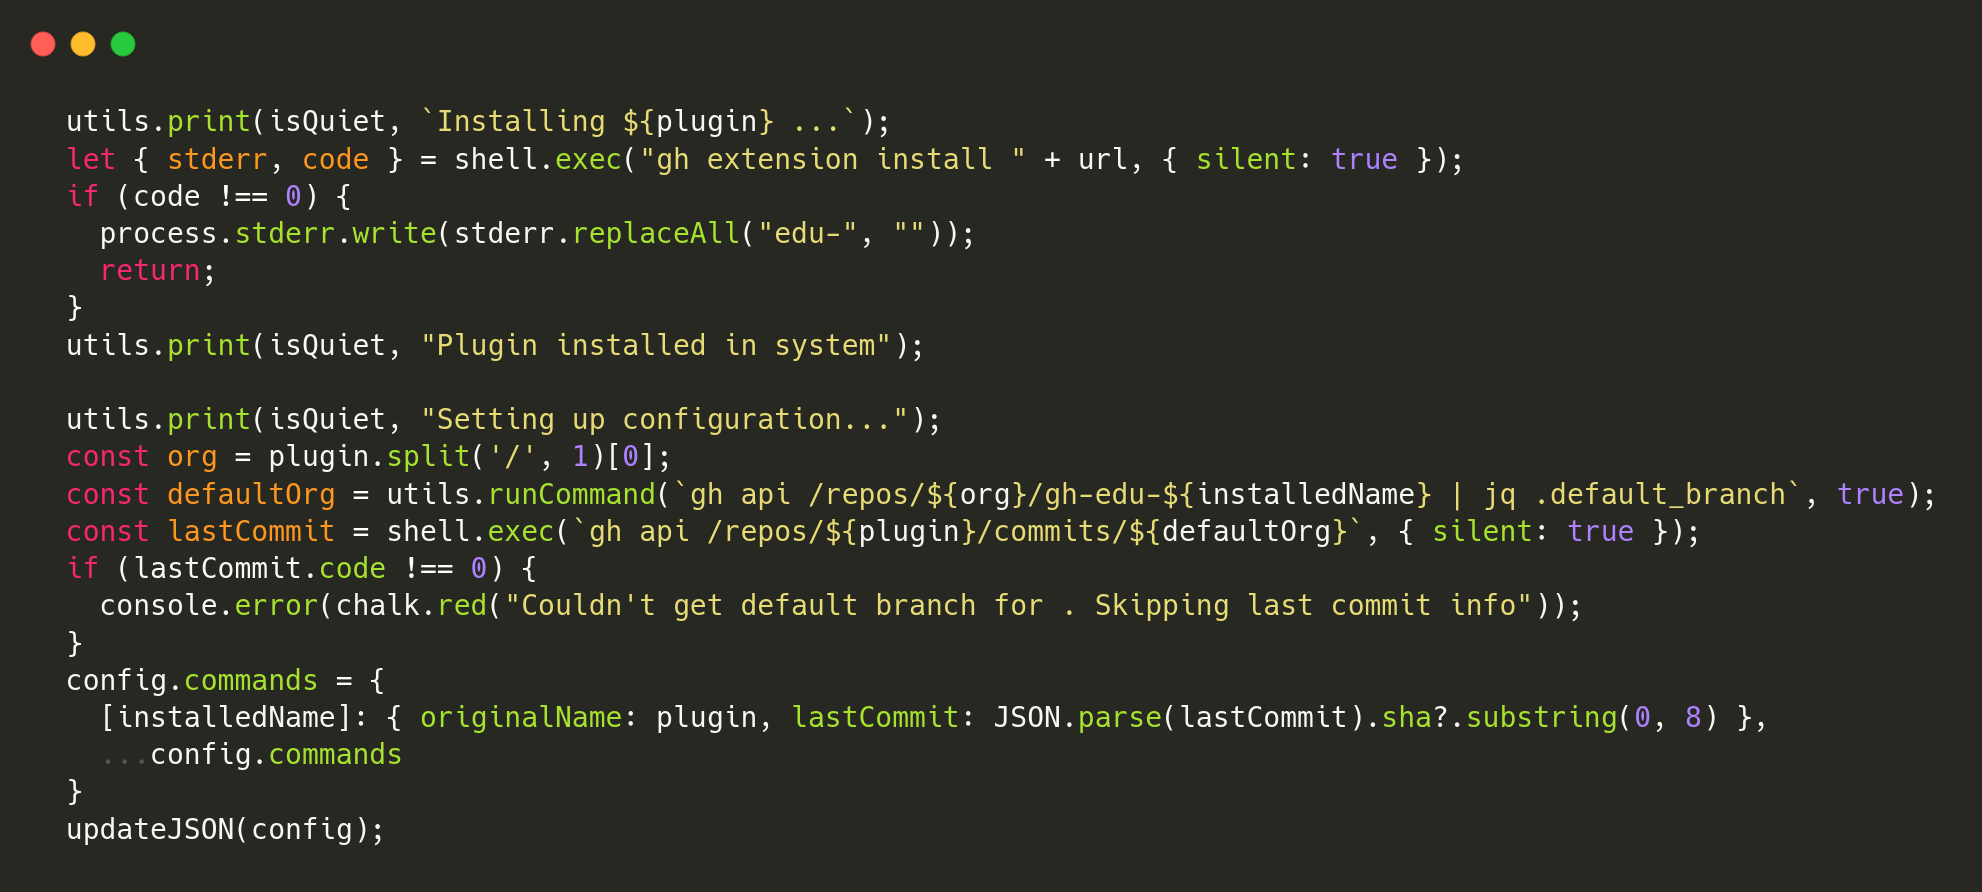
\includegraphics[width=\textwidth]{images/installCode.png}}
    \caption{Implementación. Código para instalar extensiones}
    \label{fig:installCode}
\end{figure}

En la figura \ref{fig:installCode} vemos que después de instalar la extensión, hacemos una llamada \emph{API REST} para saber cuál es la rama por defecto. Al tener esta información, podemos buscar cuál es el \gls{hash} del último \emph{commit}, para actualizar el campo \verb|lastCommit|.

\emph{Nota: utils.print() es una función muy simple para determinar si el mensaje debería imprimirse o no, dependiendo del valor del flag --quiet}.

Para que \verb|commander| acepte únicamente las extensiones instaladas, se ha escrito el siguiente código (figura \ref{fig:addThirdParty}):

\begin{figure}[H]
    \centering
    \makebox[\textwidth][c]{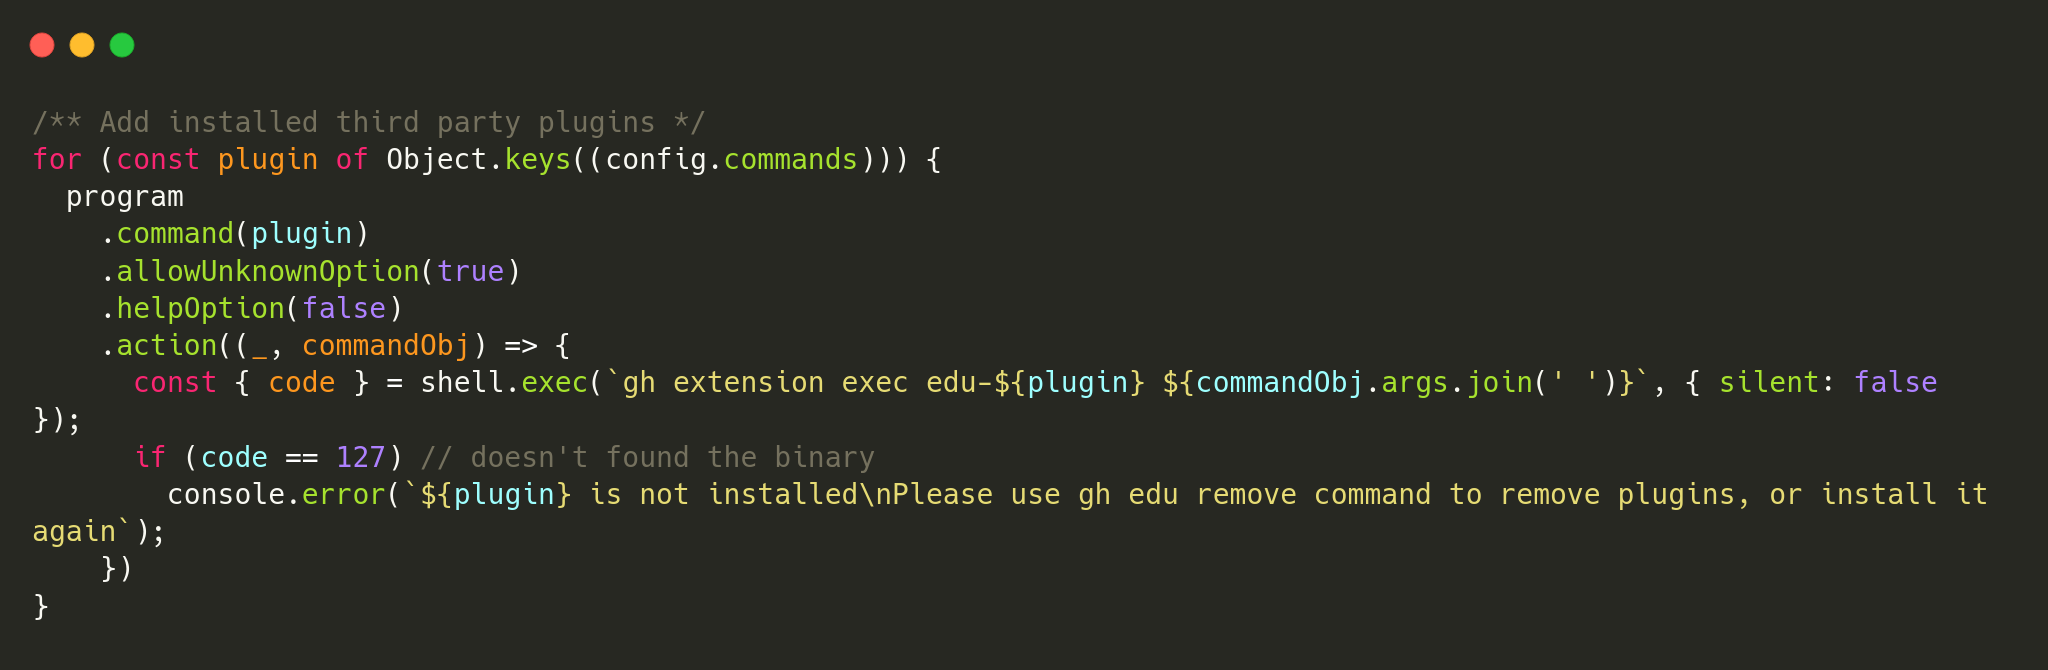
\includegraphics[width=\textwidth]{images/addThirdParty.png}}
    \caption{Implementación. Controlador. Añadir extensiones third-party}
    \label{fig:addThirdParty}
\end{figure}

Todas las extensiones, que se hayan instalado en el sistema a través de \verb|gh-edu|, se añadirán como comandos disponibles. También se activa la posibilidad de usar opciones desconocidas y se delega su gestión al subcomando en cuestión. Así mismo se desactiva la ayuda y en el manejo de errores solo se comprueba que el comando haya sido ejecutado, pues naturalmente de estas tareas se tiene que ocupar cada extensión.

Aquí se deja ver la madurez del programa al permitirnos utilizar comandos desconocidos, función que, al momento de escribir estas líneas, todavía no es posible con \href{https://github.com/spf13/cobra/issues/739}{cobra}.

\subsection{Manejo del único punto de información: data.json} \label{impl:data.json}
Lo primero que el programa hace al ser ejecutado, es comprobar la validez del fichero. La siguiente figura (\ref{fig:dataGraph}) muestra los estados por los que se pasa para lograrlo.

\begin{figure}[H]
    \centering
    \makebox[\textwidth][c]{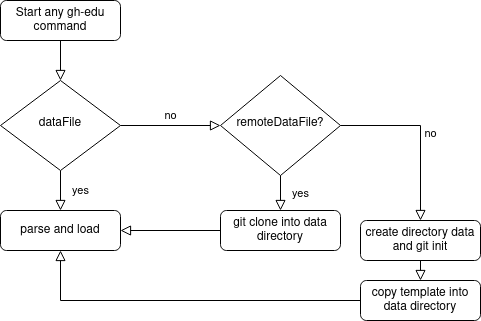
\includegraphics[width=0.5\textwidth]{images/createConfig.png}}
    \caption{Obtención del archivo data.json}
    \label{fig:dataGraph}
\end{figure}

Es primer paso es comprobar si se encuentra en la localización correspondiente (\verb|~/.config/gh-edu/data.json|). De no ser así, se intenta conseguirlo desde el repositorio \verb|gh-edu-profile|. Como última instancia se crea un fichero nuevo, partiendo de una plantilla que contiene todos los campos necesarios.

Sabiendo que el fichero está disponible, pasamos a validar su contenido. Primero se \glspl{deserialization} para comprobar que es un fichero JSON válido. Acto seguido pasamos a realizar una comprobación simple de los campos, comprobando que estén en el fichero y que las \glspl{regex} sean válidas.

\begin{figure}[H]
    \centering
    \makebox[\textwidth][c]{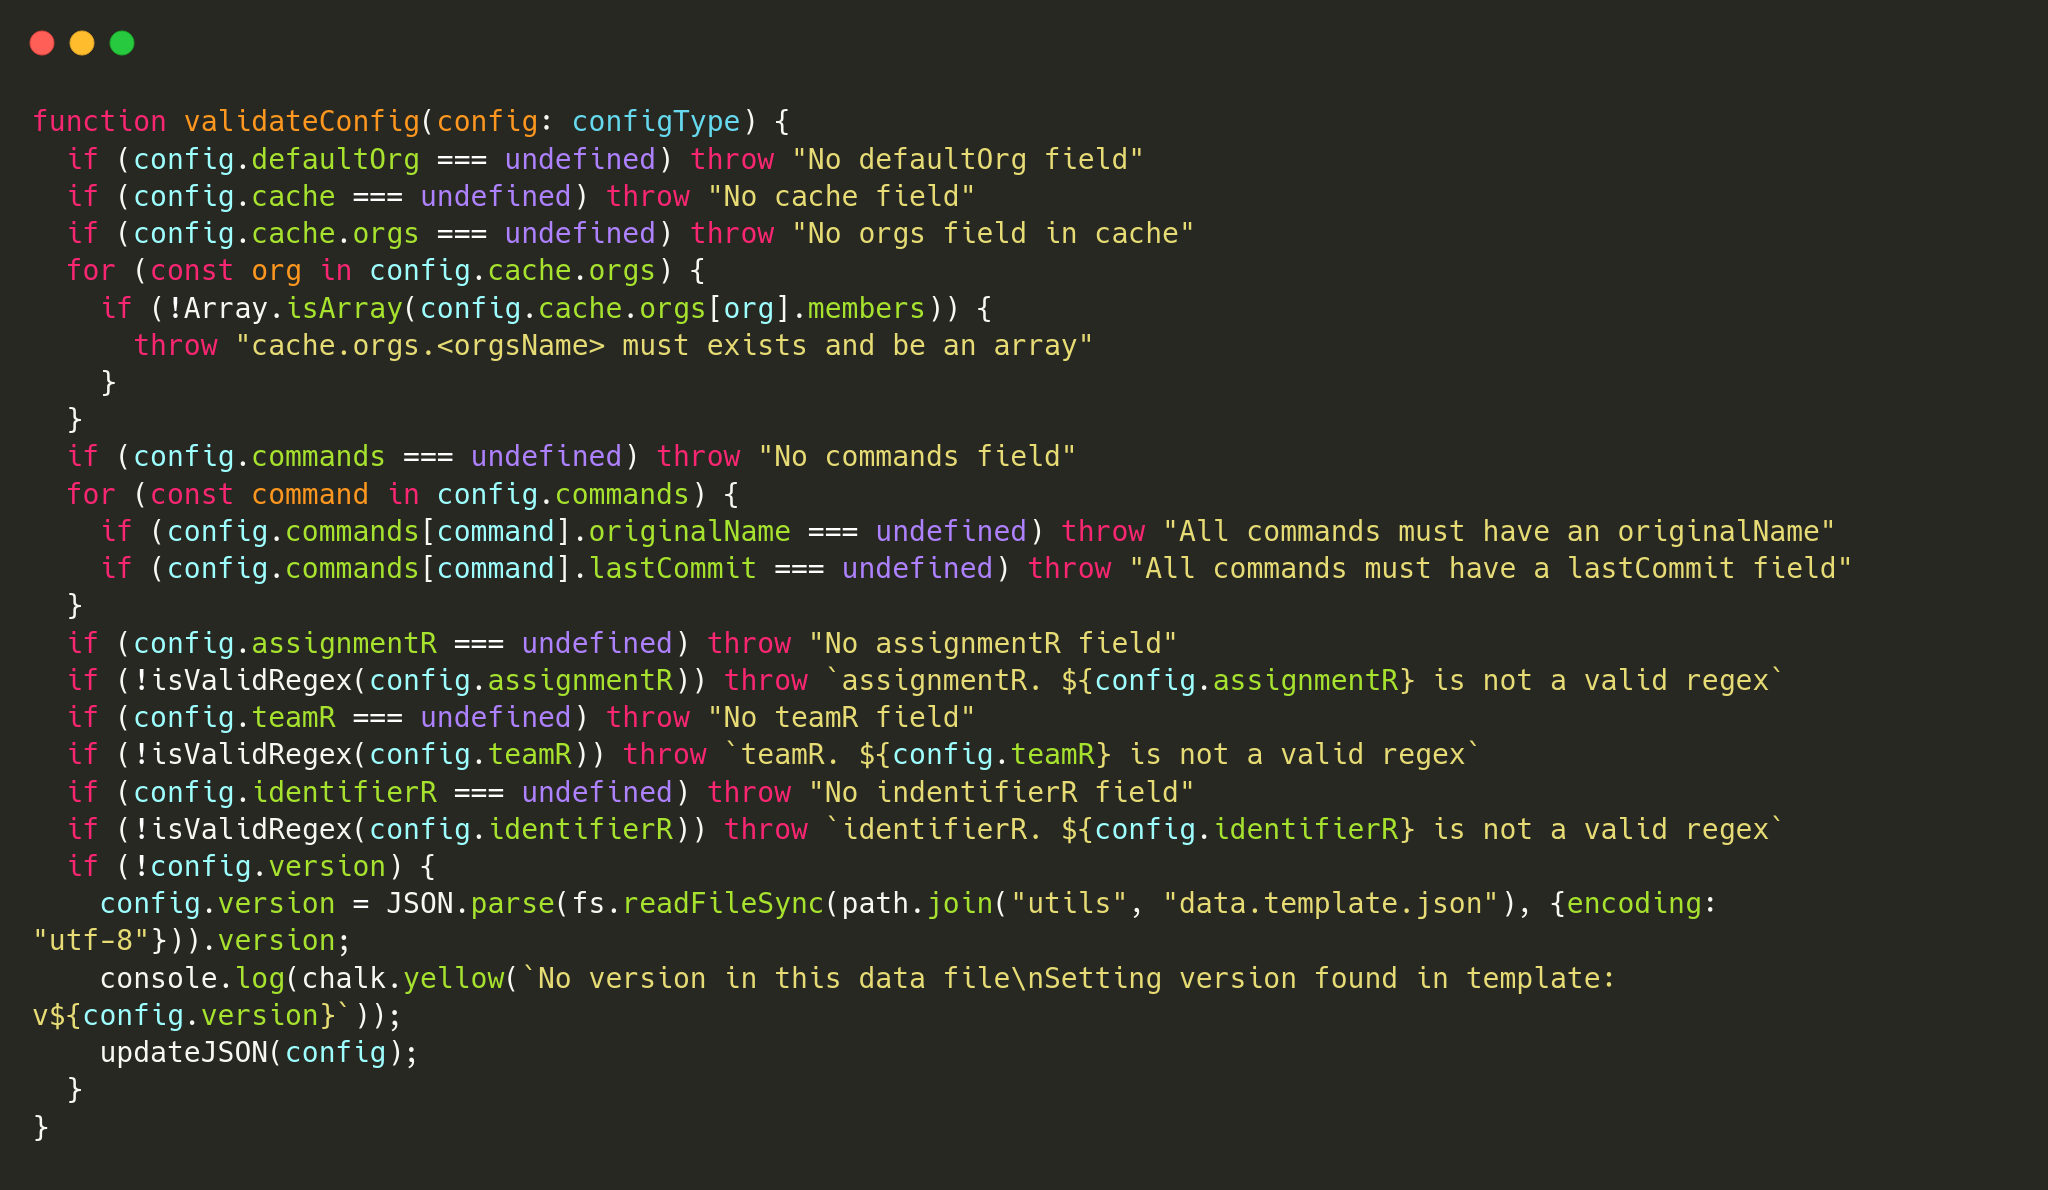
\includegraphics[width=\textwidth]{images/comprobacion.png}}
    \caption{Implementación. data.json. Comprobamos que los campos son válidos}
    \label{fig:comprobar}
\end{figure}

Cada vez que se quiera actualizar la información, se actualiza la variable donde se cargó el fichero, se \glspl{serialization} y se escribe de vuelta al fichero.

\section{Extensión minimalista: {\tt gh-edu-view}}\label{sec:gh-edu-view-implementation}

A la hora de escribir una extensión para \verb|gh-edu| en \verb|JS|, se procede de la misma forma que con una extensión \verb|gh|.
Deben crearse los ficheros \verb|gh-edu-view/gh-edu-view| (script bash) y \verb|gh-edu-view/gh-edu-view.js| (programa \verb|JS|).

Para intentar conseguir los identificadores relacionados a los alumnos, con nada más que la información proporcionada con GitHub, no nos queda otra opción que buscar en todos los campos, donde dicha información podría estar disponible, y devolver un \emph{array} con todos los posibles resultados.

\begin{figure}[H]
    \centering
    \makebox[\textwidth][c]{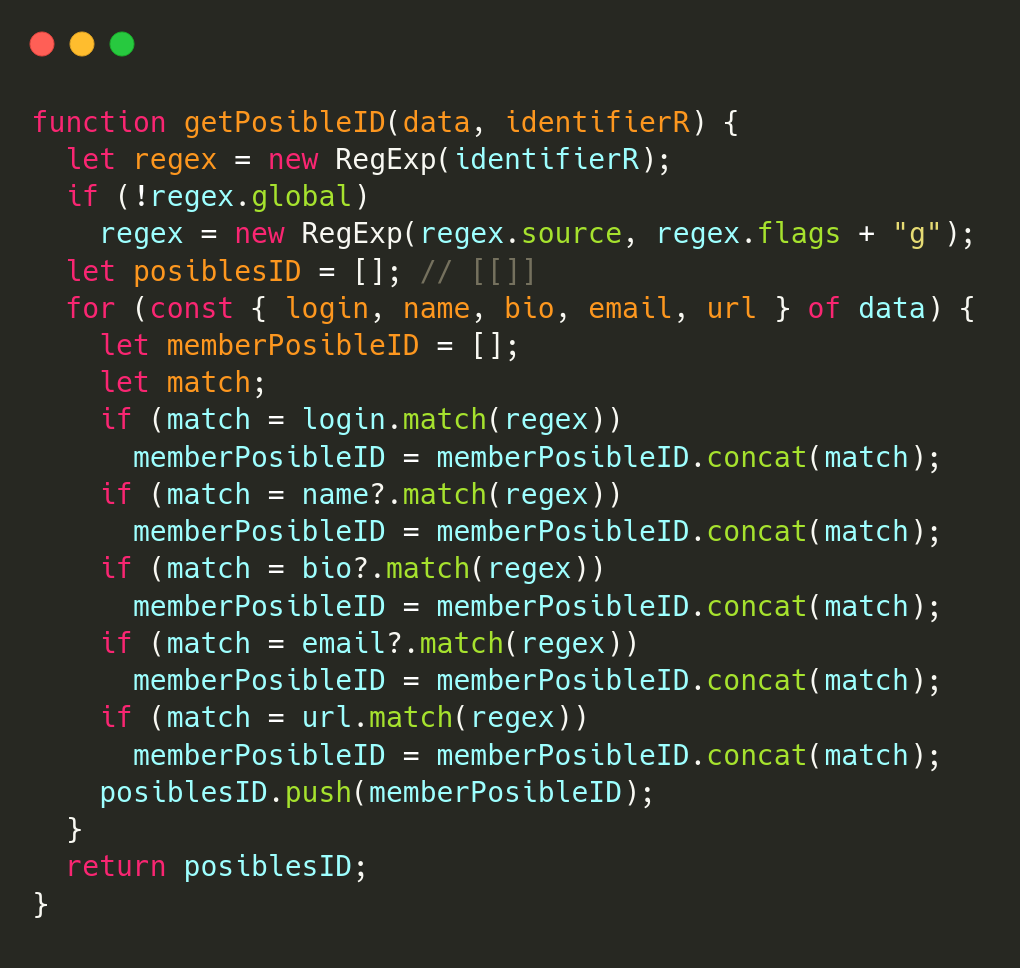
\includegraphics[width=0.5\textwidth]{images/posibleID.png}}
    \caption{Implementación. gh-edu-view. Obtención de posibles identificadores}
    \label{fig:viewId}
\end{figure}

Toda la información proporcionada por el comando \verb|members| se puede conseguir con una simple petición en GraphQL (figura \ref{fig:viewQuery}).

\begin{figure}[H]
    \centering
    \makebox[\textwidth][c]{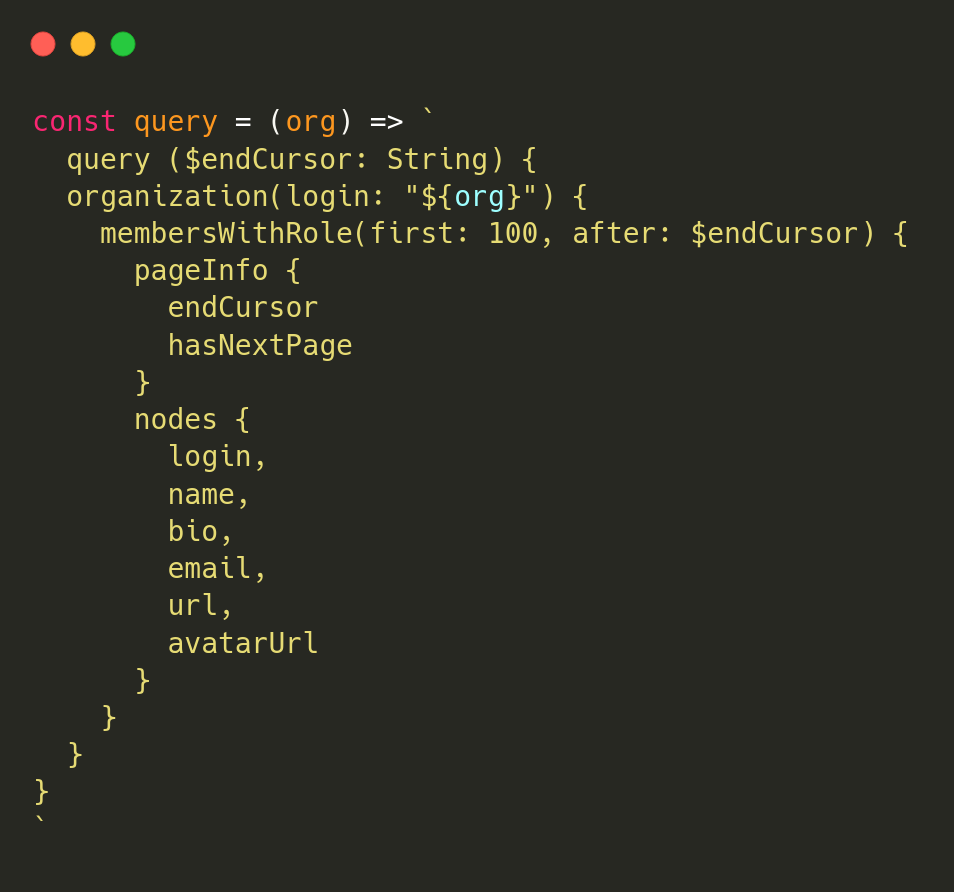
\includegraphics[width=0.5\textwidth]{images/view-query.png}}
    \caption{Implementación. gh-edu-view. Petición para conseguir diversos campos de cada alumno}
    \label{fig:viewQuery}
\end{figure}

\section{{La librería \tt shelljs} y el manejo de E/S: {\tt gh-edu-data}} \label{impl:gh-edu-data}
Uno de los defectos de \verb|shelljs| que ya se ha comentado en el apartado de \textbf{Tecnologías} (\ref{shelljs}) es como no permite el uso de \verb|STDIN| o tuberías. Algo importante en este proyecto, pero especialmente en esta extensión por el uso avanzado de \verb|fzf| y \verb|jq|. Estas dos tecnologías, a pesar de ser completamente independientes la una a la otra, pueden trabajar conjuntamente gracias a su diseño flexible y minimalista a través de tuberías, haciendo posible la previsualización dinámica de los elementos en el comando \verb|log| (figura \ref{fig:interface-log})

Este comportamiento es requerido, ya que no es posible pasar un objeto \verb|JS| o un \emph{array} al input de un programa que todavía no ha sido ejecutado. Solo se puede usar cadenas de texto. Lo ideal es ejecutar el comando, y de forma asíncrona ir procesando la estructura de datos, enviando cadenas de texto, como se hace en \verb|gh-edu-plagiarism| (gracias a \href{https://pkg.go.dev/os/exec@go1.18.3#Cmd.StdinPipe}{cmd.StdInPipe}).

Hasta que la \href{https://github.com/shelljs/shelljs/issues/424}{incidencia 424} no sea resuelta, se ha tenido que realizar una solución alternativa utilizando ficheros temporales. La idea consiste en formatear el objeto o \verb|array| y escribir el resultado en un fichero, de esta forma podemos leer el fichero y transmitir esa información por medio de una tubería a otro comando en el mismo momento en el que se ejecuta el comando.

\section{Concurrencia con Go y CSP: {\tt gh-edu-plagiarism}} \label{diseño:gh-edu-plagiarism}
A diferencia del resto de extensiones \verb|plagiarism| está implementado en Go. Uno de los motivos del cambio de lenguaje es demostrar como se puede desarrollar extensiones en cualquier lenguaje sin muchas dificultades.

También, como se comentó en \textbf{Tecnologías} (\ref{go}) este programa es altamente concurrente y paralelo. Go cuenta con un modelo de concurrencia bastante particular basado en el trabajo teórico de Tony Hoare \emph{Communicating Sequential processes} (CSP) \cite{hoare1985communicating}.

Para entender las explicaciones de esta sección es necesario conocer dos conceptos: las gorutinas y los canales. Las gorutinas son \glspl{corrutine} independientes que se ejecutan en hilos verdes (\emph{green threads}), los cuales son hilos emulados generados en tiempo de ejecución, estos hilos se multiplexan a hilos reales del procesador a través del \verb|Go scheduler|, que determina cuanto tiempo debe estar cada hilo verde consumiendo CPU.

Los canales son la estructura de datos que nos permite enviar información de una gorutina a otra y también sirven de elemento sincronizador, cuando se envía un elemento, la gorutina no continua hasta que el otro lado (el emisor) haya recibido la información y viceversa.

La explicación de la figura \ref{fig:plagiarism} en términos de código sería la siguiente:\\
Cada bloque dentro del módulo \verb|Concurrent| es una gorutina que se ejecuta de forma independiente y cada flecha pertenece a un canal, que sincroniza y a su vez transmite información de una gorutina a otra.

La gorutina \verb|clone| va creando a su vez gorutinas a medida que más repositorios se vayan filtrando. Debido a que las gorutinas apenas consumen recursos, está bien eliminar y crear tantas como queramos. No obstante, como estamos realizando programación paralela, tenemos que tener cuidado de que no haya muchas más gorutinas corriendo que núcleos disponibles en el procesador, pues entonces conseguiríamos el efecto contrario al deseado, ralentizando toda la aplicación debido al constante cambio de contexto entre hilos. Para limitar la creación de gorutinas al número de núcleos disponibles se ha utilizado un semáforo. Un semáforo es una variable o estructura de datos que permite una cantidad arbitraria de procesos. Un semáforo binario es a efectos prácticos un \verb|lock| o \verb|mutex|.

\begin{figure}[H]
    \centering
    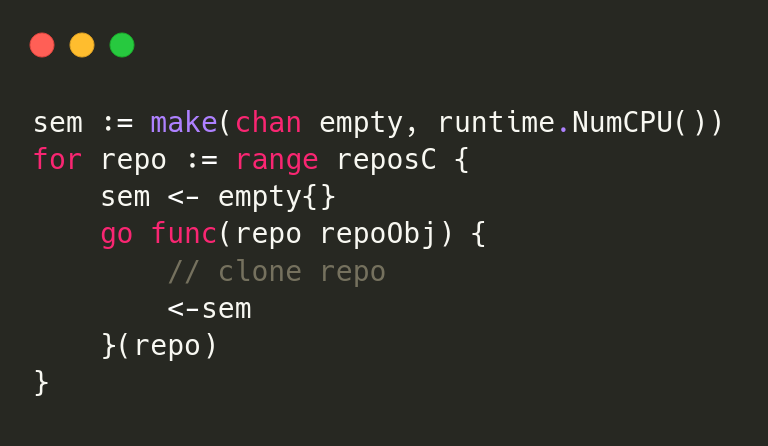
\includegraphics[width=0.5\linewidth]{images/concurrency-go.png}
    \caption{Paralelismo limitado con un sémaforo}
    \label{fig:concurrencyGo}
\end{figure}
El código que lo implementa (figura \ref{fig:concurrencyGo}) ha sido simplificado para explicar el funcionamiento del paralelismo y el semáforo.

El canal \verb|sem| es un canal con buffer, esto quiere decir que no para el flujo (no sincroniza) hasta que el buffer se llene. El tamaño de dicho buffer es \verb|runtime.NumCPU()| que retorna el número de núcleos disponibles al ejecutar el programa. En cada iteración del bucle \verb|repo| contiene un nuevo repositorio proveniente del módulo \verb|Filter| y enviamos un elemento al canal \verb|sem|, el elemento en cuestión es irrelevante, estamos usando el canal por sus propiedades de sincronización, no para la transferencia de datos. Después ejecutamos una gorutina anónima que se encarga de clonar el repositorio, cuando termine escucha y descarta del canal \verb|sem|.

De esta forma, si \verb|sem| está lleno significa que ya hay tantos procesos ejecutándose como núcleos hay disponibles, por lo que el programa queda en espera hasta que quede un hueco en el semáforo.

% Esto va en diseño. Otro de los motivos por los cuales se eligió Go es que a la hora de diseñar la extensión me percate de que el programa sería altamente concurrente y paralelo. Uno de los motivos por los cuales se creó Go fue para poder aprovechar al máximo los varios núcleos que suele tener cualquier dispositivo moderno. Así, las instituciones educativas que reutilizan la misma organización para una misma asignatura a lo largo de varios años, y por ende tienen muchos repositorios y miembros, no verán su experiencia lastrada. También se tuvo en cuenta que Go tiene soporte de primera clase con \verb|gh| y uno de los casos de uso más comunes del lenguaje son aplicaciones CLI.

\begin{figure}[H]
    \centering
    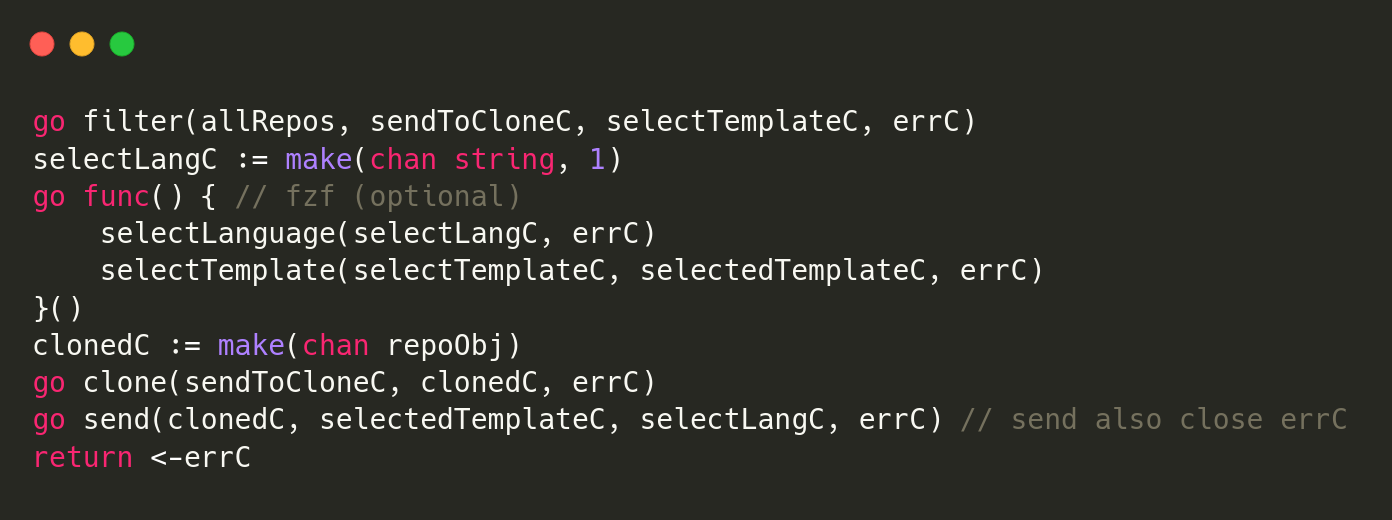
\includegraphics[width=\linewidth]{images/go-code.png}
    \caption{Código general de plagiarism}
    \label{fig:goCode}
\end{figure}

 